\documentclass{article}

\usepackage[margin=1in]{geometry} 
\usepackage{amsmath, amsthm, amssymb, amsfonts}
\usepackage{fancyhdr, graphicx, xcolor}
\usepackage{mdframed, indentfirst, minted, multicol}
\usepackage[shortlabels]{enumitem}
\usepackage{indentfirst, hyperref}
\usepackage[sorting=none]{biblatex}
\usepackage{pgfplots}
\pgfplotsset{compat=1.12}
\usetikzlibrary{decorations.text}

\pagestyle{fancy}
\addbibresource{references.bib}
\bibliographystyle{unsrt}
\renewcommand{\footrulewidth}{0.8pt}
\hypersetup{
    colorlinks=true,
    linkcolor=blue,
    filecolor=magenta,      
    urlcolor=blue,
}

\newenvironment{problem}[2][Problem]
    { \begin{mdframed}[backgroundcolor=gray!20] \textbf{#1 #2} \\ }
    { \end{mdframed} }
\newenvironment{solution}{\textbf{Solution}}

\lhead{\textbf{Pitch: The Holy Grail of Computer Acoustics}}
\rfoot{Walford Prize 2022}

\begin{document}
\makeatletter
    \begin{titlepage}
        \begin{center}
	   % { \includegraphics[width=12cm]{nameofpicture.jpg} }
	   {\ \\ \ \\}
        \vbox{}\vspace{5cm}
            {
                \Large Walford Prize 2022, Charterhouse School \\[0.5cm]
                \bf\Large Pitch: The Holy Grail of Computer Acoustics
            } \\ [3cm] 
            {\large Hongming (Lancelot) Liu \\}
            {\large 1.2.7$\alpha$ \\}
        \end{center}
    \end{titlepage}
\makeatother

\section{Introduction}

Computers have become increasingly powerful, and people have become progressively lazy. Where musicians would sit in the concert hall and transcribe every note they heard, where stenographers type at unfathomable speeds, people seek easier, cheaper, faster solutions.

In the world of music and acoustics, this resulted in constructs like the Fourier Transform (FT) and the Fast Fourier Transform (FFT). Suddenly, computers could speak and hear like humans and easily synthesise instruments' sounds. These were the precursors of the voice of Siri, and EDM, among others.

Then came the storm that is artificial intelligence. Suddenly, this imitation of human intelligence could perform tasks for us. From the black box that is the YouTube algorithm to the auto-correct that fixes your spelling for you, machine learning has drastically improved the capabilities of computers.

However, one thing continues to elude the progression of computerisation. Processing music and transcribing pitch, simply the frequency of air molecules' vibration, remains an essential research topic. 

\subsection{Pitch}

\emph{Pitch} is a human construct invented to help us categorise sounds: pitch is simply the frequency of sounds. Most of the world uses a 12-tone equal temperament system (12-TET), where each musical octave is divided into 12 semitones. Each is assigned a name, for example, in the English system, using the alphabet from A to G. There are other methods of defining musical pitch, such as the 24-tone equal temperament used by the Arabs. Still, for ease of comparison, only the standard Western system of 12-TET will be discussed.

The system is logarithmic, where an increase by one octave signifies a pitch doubling, and a decrease by one octave represents a pitch halving. For example, where A$_4$ is $440$Hz, A$_5$, one octave above, would be $880$Hz. The separation into $12$ divisions and the factor of $2$ every octave mean that the ratio between successive semitones is $\sqrt[12]{2}$. Hence, a nifty little equation can be used to find the frequency of any note compared to a reference note.

\begin{align*}
    f_n & = f_0 (\sqrt[12]{2})^n \\
\end{align*}

Where $f_0$ is the frequency of a reference note, most commonly $A_4$ with a frequency of $440$Hz, and $n$ is the number of semitones from the reference tone. A higher note than the reference would use a positive $n$, and a lower note would use a negative $n$.

Using this, one could demonstrate the doubling effect described previously. To calculate the frequency of A$_5$, one octave or twelve semitones above the reference A$_4$:

\begin{align*}
    f_{12} & = (440) (\sqrt[12]{2})^{12} \\
    & = 880 \\
\end{align*}

\subsection{Pitch... Detection}

Herein lies the problem. There are situations where one would want to transcribe said pitches. Whether that be a guitarist using their phone to tune their instrument, or a researcher, needing to turn a vast catalogue of songs into digitised sheet music to train their models with.

Humans have a seemingly innate ability to sense pitch and many other attributes of the sound around us\cite{Oxenham2012PitchPerception}. Many can even precisely pinpoint a sound they hear without reference, known as Absolute Pitch. Even those who don't can still perceive much information, such as timbre, intervals, keys, and more\cite{Deutsch2013AbsolutePitch}. Computers, on the other hand, are not so lucky. An entire field of study is dedicated to processing auditory signals, and to this day, extracting any information from music, or sounds, in general, is a significant area of research.

The problem in this essay arises: how to extract information about pitch from raw audio?

In this essay, the words \emph{pitch} and \emph{frequency} are used interchangeably.

\section{Theoretical Waves}

Let's first consider the simplest case to move on to more complicated methods of extracting pitch.

\begin{problem}{1}

Find the frequency of this signal. \\
    
\begin{tikzpicture}
    \begin{axis}[
        width = 0.9\textwidth, height = 5cm,
        axis lines = left, smooth,
        xlabel = \(Time / s\),
        ylabel = {\(Amplitude\)}, ytick distance = 1,
        grid=both, minor tick num = 0
        grid style = {line width = .1pt, draw = gray!10},
        major grid style = {line width = .2pt,draw = gray!50},
    ]
    \addplot[
        domain = 0:10, 
        samples = 100
    ]{sin(deg(pi*x))};
    \addlegendentry{\(\text{Signal} f(t)\)}
    \end{axis}
\end{tikzpicture}

\end{problem}

The signal here has a period of $2$ seconds: it repeats itself every $2$ seconds. Hence the frequency is $0.5$Hz. In fact, this signal is simply the function $f(t) = \sin(\pi t)$. Things become more complicated when the signal is no longer one function. In real life, the sounds we recognise as speech, instruments, and other objects are not pure waves but a combination.

\begin{problem}{2}

Find the frequency of this signal. \\
    
\begin{tikzpicture}
    \begin{axis}[
        width = 0.9\textwidth, height = 5cm,
        axis lines = left, smooth,
        xlabel = \(Time / s\),
        ylabel = {\(Amplitude\)}, ytick distance = 1,
        grid=both, minor tick num = 0
        grid style = {line width = .1pt, draw = gray!10},
        major grid style = {line width = .2pt,draw = gray!50},
    ]
    \addplot[
        domain = 0:0.02, 
        samples = 400
    ]{sin(deg(880*pi*x)) + sin(deg(888*pi*x))};
    \addlegendentry{\(\text{Signal} f(t)\)}
    \end{axis}
\end{tikzpicture}

\end{problem}

This signal is the combination of two sine waves. Thus, finding the frequency is not as straightforward as using the equivalence relationship $f(t) = A\sin(2\pi f + \phi)$, where we could simply read off the value of $f$, the frequency. Fortunately, all the component waves are of the same amplitude and phase. Coincidentally, they also result in a perceivable pitch with a \emph{beat}. 

\begin{tikzpicture}
    \begin{axis}[
        width = 0.9\textwidth, height = 4cm,
        axis lines = left, smooth,
        xlabel = \(Time / s\),
        ylabel = {\(Amplitude\)}, ytick distance = 1,
        grid=both, minor tick num = 0
        grid style = {line width = .1pt, draw = gray!10},
        major grid style = {line width = .2pt,draw = gray!50},
    ]
    \addplot[
        domain = 0:1, samples = 400, color = black
    ]{sin(deg(880*pi*x)) + sin(deg(890*pi*x))};
    \addlegendentry{\(\text{Signal} f(t)\)}
    \addplot[
        domain = 0:1, samples = 400, color = red
    ]{sin(deg(880*pi*x)};
    \addlegendentry{\(\text{Sine Wave 440Hz}\)}
    \addplot[
        domain = 0:1, samples = 400, color = pink
    ]{sin(deg(888*pi*x)};
    \addlegendentry{\(\text{Sine Wave 444Hz}\)}
    \end{axis}
\end{tikzpicture}

We can work out the frequency of the fundamental tone using some maths. First, we introduce this trigonometric identity.

\begin{align*}
    \sin\alpha + \sin\beta & = 2\cos\left( \frac{\alpha - \beta}{2} \right)\sin\left( \frac{\alpha + \beta}{2} \right)
\end{align*}

We have two sine waves to add, namely:

\begin{align*}
    f(t) & = \sin(2\pi(400) x) \\
    g(t) & = \sin(2\pi(444) x) \\
    f(t) + g(t) & = 2\cos\left( \frac{2\pi(444 - 440)}{2}t \right)\sin\left( \frac{2\pi(444 + 440)}{2}t \right) \\
    & = 2\cos(4\pi t)\sin(884\pi t) \\
\end{align*}

From this, we can conclude that the addition of the two signals of $440$Hz and $444$Hz results in a signal of $442$Hz, illustrated by the $\sin$ portion of the result and an overall beat that sounds like... \emph{waaaaaah... waaaaaah...}, with a frequency of $2$Hz. 

Many further complications can be added to this mix: varying the amplitudes and phase, adding more fundamental signals, introducing noise, and so on. Using pure mathematics to determine the characteristics of an incoming signal quickly becomes impractical. 

Here is an example with three sine waves (of the same amplitude), with significant frequency differences and some added \emph{noise}. Just as air resistance is the secret trap of projectile motion, noise is the enemy of all acousticians (and music lovers).

\begin{problem}{3}

Find the frequency of this noisy signal.

\begin{tikzpicture}
    \begin{axis}[
        width = 0.9\textwidth, height = 5cm,
        axis lines = left, smooth,
        xlabel = \(Time / s\),
        ylabel = {\(Amplitude\)}, ytick distance = 1,
        grid=both, minor tick num = 0
        grid style = {line width = .1pt, draw = gray!10},
        major grid style = {line width = .2pt,draw = gray!50},
    ]
    \addplot[
        domain = 0:0.02, samples = 400, color = black
    ]{sin(deg(500*pi*x)) + sin(deg(1000*pi*x)) + sin(deg(1500*pi*x)) + 0.5*rand};
    \addlegendentry{\(\text{Signal} f(t)\)}
    \end{axis}
\end{tikzpicture}

\end{problem}

The signal here is a mixture of many other signals. Specifically, this one combines waves of $250$Hz, $500$Hz, and $750$Hz. This example is simple enough that at a glance, we can ascertain that the period of the overall waveform is $0.4 * 10^{-2}$ seconds, and therefore the frequency of the overall signal is $250$Hz. But for demonstrative purposes, let us try to work it out analytically.

First, with the almighty power of \emph{being the person who wrote the question}, noise is removed. The problem is simplified to:

\begin{align*}
    & \sin(500\pi t) + \sin(1000\pi t) + \sin(1500\pi t) \\
    & = ... \quad \text{I give up.}
\end{align*}

\section{Algorithmic Approaches}

Over the past decades, there have been better methods to extract pitch information from a signal than using trigonometric identities: least of all because \textbf{we do not have the component signals} in the real world!

\subsection{Fourier Transform}

The Fourier (Integral) Transform is very efficient function which can disassemble a signal into its components. Namely, it is an equation that looks like this:

\begin{align*}
    \hat{f}(\zeta) & = \int_{-\infty}^{\infty} f(x) e^{-2i\pi\zeta x} \text dx \\
\end{align*}

FT does one thing to extract component signals: given a smoothie; it returns the recipe\cite{AnTransform}. The complicated integral can be transformed into something more intuitive:

\begin{align*}
    X_k & = \sum_{n=0}^{N-1} x_n e^{\frac{2\pi ink}{N}}
\end{align*}

The idea is that any function, no matter how complicated or how weird, can be separated into a (possibly infinite) series of sine waves, even functions that seem to have no relevance to a sine wave, such as $f(x) = x^2$. In the world of signal processing, that means any incoming signal and be disassembled into many component signals in the form of $f(t) = A\sin(2\pi nf + \phi)$.

In the above equation, at any frequency $X_k$, the magnitude of this component is the sum, $\sum_{n=0}^{N-1}$, of the contributions to this frequency at any time, $x_n e^{\frac{2\pi ink}{N}}$. 

This leads on to another analogy for FT: 

\begin{center}
    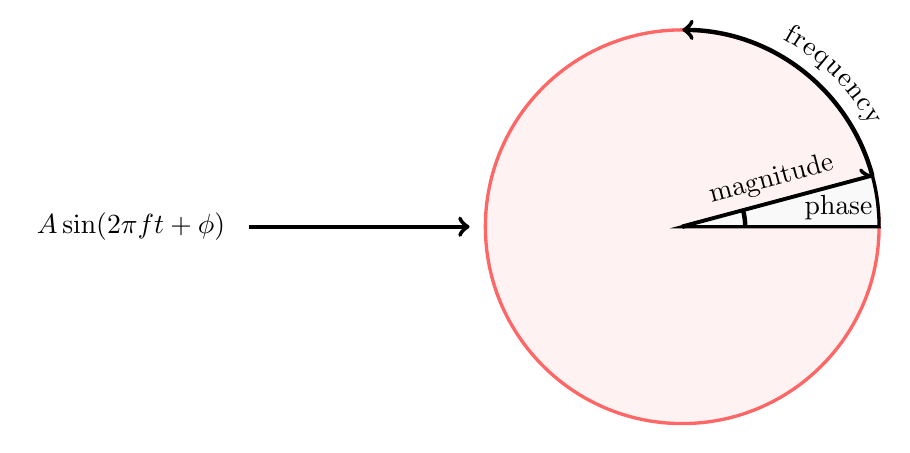
\begin{tikzpicture}
        \filldraw[color=red!60, fill=red!5, very thick] (0,0) circle (2.5);
        \draw[decoration={text along path,
                text={magnitude}, text align={center}, raise=0.2cm}, decorate] (0:0) -- (15:2.5);
        \draw[ultra thick, ->] (0:0) -- (15:2.5);
        \draw[decoration={text along path,
                text={frequency}, text align={center}, raise=0.2cm}, decorate] (90:2.5) arc (90:0:2.5);
        \draw[ultra thick, ->] (15:2.5) arc (15:90:2.5);
        \draw[fill=gray!5, very thick] (0:0) -- (0:2.5) arc (0:15:2.5) -- cycle;
        \draw[ultra thick] (0:0.8) arc (0:15:0.8);
        \node at (7:2) {phase};
        
        \node at (180:7) {$A\sin(2\pi ft + \phi)$};
        \draw[ultra thick, ->] (180:5.5) -- (180:2.7);
    \end{tikzpicture}
\end{center}

Imagine every component signal as a \emph{circular path}: something that moves along a circle with a certain radius (magnitude), starting at an offset angle (phase), at a certain speed (frequency). 

Taking a closer look at the formula, specifically $e^{\frac{2\pi ink}{N}}$, one notices that the result is complex. The complex value makes sense since, in this form, a complex number describes  a radius (the magnitude) and an angle (the phase) at  any frequency. (Computers often cannot handle calculations involving pure complex numbers, and the Cartesian equivalents of the results must be used.)

With this in mind, we can use the FT on the noisy signal in \textbf{Problem 3}. Such calculations should not be attempted by hand - much like calculators are used in problems involving the normal distribution, computers are used to do the heavy lifting with FT. 

For curiosity's sake, here's how maths becomes code:

\begin{minted}[mathescape, linenos]{python}
from scipy.fftpack import fft
from matplotlib import pyplot as plt
from scipy.io import wavfile
import numpy as np
import scipy
\end{minted}

After importing all the required libraries, we extract the audio file.

\begin{minted}[mathescape, linenos]{python}
fs_rate, signal = wavfile.read("250+500+750+noise.wav")\footnote{For this file and others, see the last section.}

if len(signal.shape) == 2: signal = signal.sum(axis = 1) / 2
samples = signal.shape[0]
seconds = samples / float(fs_rate)
step = 1.0 / fs_rate
timeVector = scipy.arange(0, seconds, step)
\end{minted}

Fortunately, the bulk of the algorithm has already been expertly created by the maintainers of \texttt{scipy}.

\begin{minted}[mathescape, linenos]{python}
FFT = abs(fft(signal))
FFTPositive = FFT[range(int(samples / 2))]
freqs = scipy.fftpack.fftfreq(signal.size, timeVector[1] - timeVector[0])
\end{minted}

Once the transform has been completed, it is important to note that the algorithm also deals with \emph{negative frequencies}: this is not an issue since signals are symmetrical. Half of the values are removed, and the data for $0$ to $1600$Hz is taken.

\begin{minted}[mathescape, linenos]{python}
FFTFreqsPositive = freqs[range(int(samples / 2))] 

plt.plot(FFTFreqsPositive[:50000], abs(FFTPositive[:50000]), "b")
plt.xlabel('Frequency (Hz)')
plt.ylabel('Positive Count')
plt.show()
\end{minted}

\begin{center} \includegraphics[width=0.8\textwidth]{img/fft_figure.png} \end{center}

And indeed, the FT algorithm shows three peaks, at $250$Hz, $500$Hz, and $750$Hz, precisely as intended. However, there are reasons why researchers are no longer pursuing forms of the Fourier Transform for detecting pitch. 

This author's specific implementation took an average of $75$ms to execute \footnote{This was achieved on an M1 ARM SoC, known for its ruthless hybrid cores, with the Fast Fourier Transform (FFT) library from the Python SciPy library, which is already more efficient than the traditional definition of the Fourier Transform.}. Despite being a very short amount of time for humans, this delay makes it impractical to use FTs (or FFTs) to process large amounts of data or for real-time applications such as tuning apps on phones.

\subsection{Zero Crossings}

In an attempt to solve the problem of computational complexity, an extremely simple algorithm was conceived, which simply measures how many times the signal crosses zero. Since logically, every complete wave crosses zero twice, the frequency is simply $f = \frac{N_{\text{zcr}}}{2}$.

Counting the number of zero crossings is equally easy. Since digital audio has a finite number of samples, one need only determine if one sample and its successor multiply to give a negative number in order to find a zero crossing. In its entirety, the algorithm is\cite{Torres-Garcia2022Pre-processingExtraction}:

\begin{align*}
    N_{\text{zcr}} & = \frac{1}{N} \sum_{n=0}^{N-1} \coprod \left\{ s(n)s(n-1) < 0 \right\} \\
    f & = \frac{N_{\text{zcr}}f_s}{2} \\
\end{align*}

Where $N_{\text{zcr}}$ is the number of zero crossings, and $f_s$ is the sampling frequency of the signal, and the operator $\coprod \{A\}$ is 1 if the argument $A$ is true and $0$ otherwise.

This technique is extremely simple to implement and blazing fast. Unfortunately, it is also overly inaccurate. In the face of noise or harmonic signals, the number of zero crossings is easily disturbed. For example:

\begin{center}
    \begin{multicols}{2}
        \noindent \begin{tikzpicture}
            \begin{axis}[
                width = 0.45\textwidth, height = 5cm,
                axis lines = left, smooth,
                xlabel = \(Time / s\),
                ylabel = {\(Amplitude\)}, ytick distance = 1,
                grid=both, minor tick num = 0
                grid style = {line width = .1pt, draw = gray!10},
                major grid style = {line width = .2pt,draw = gray!50},
            ]
            \addplot[
                domain = 0:0.04, samples = 400, color = black
            ]{sin(deg(100*pi*x))};
            \addlegendentry{$f(t) = \sin(100\pi t)$}
            \end{axis}
        \end{tikzpicture}
    
        \begin{tikzpicture}
            \begin{axis}[
                width = 0.45\textwidth, height = 5cm,
                axis lines = left, smooth,
                xlabel = \(Time / s\),
                ylabel = {\(Amplitude\)}, ytick distance = 1,
                grid=both, minor tick num = 0
                grid style = {line width = .1pt, draw = gray!10},
                major grid style = {line width = .2pt,draw = gray!50},
            ]
            \addplot[
                domain = 0:0.04, samples = 400, color = black
            ]{sin(deg(100*pi*x)) + 0.3*sin(deg(1000*pi*x))};
            \addlegendentry{$f(t) = \sin(100\pi t) + \sin(1000\pi t)$}
            \end{axis}
        \end{tikzpicture}
    \end{multicols}
\end{center}

Where the example on the right has significantly more zero crossings, despite having the same fundamental frequency.

There are similar methods to zero crossings, such as counting peak rates or slope event rates. These all rely on detecting the occurence of some event within some time, i.e., Time-Event Rate Detection\cite{Gerhard2003PitchTechniques}. They will not be discussed here.

\subsection{Autocorrelation}

Autocorrelation is the comparison of something to itself. In the case of signal processing, this means comparison against self at a different time, or \emph{lag}, typically denoted $\tau$.

The autocorrelation function at any given value of lag $\tau$ is given by\cite{Amado2008PitchNotes}:

\begin{align*}
    \phi(\tau) & = \frac{1}{N} \sum_{n=0}^{N-1} S(t)S(t-\tau) \\
\end{align*}

Where $S(n)$ is the signal at any given time $t$, and $N$ is the total number of samples within the current window of observation. For any pure tone, the function exhibits peaks at lags corresponding to the period and its integer multiples. 

Again, it is wildly impractical to carry out this calculation by hand. The below computations are again run on the waveform in \textbf{Problem 3}.

\begin{minted}[mathescape, linenos]{python}
import librosa
import numpy as np
import scipy
import matplotlib.pyplot as plt

data, sampleRate = librosa.load('250+500+750+noise.wav')
r = librosa.autocorrelate(data, max_size=10000)
\end{minted}

When the result of the autocorrelation is plotted, there is one maximum at $0$, signifying that the signal is exactly similar to itself when not phase shifted. Another peak exists a certain value of $\tau$ away, and every integer multiple after that. 

\begin{center} \includegraphics[width=0.8\textwidth]{img/ac_figure.png} \end{center}

Given that these peaks signify the period of the target frequency:

\begin{minted}[mathescape, linenos]{python}
# Eliminate unlikely ranges of pitches
r[:int(sampleRate/librosa.midi_to_hz(120))] = 0
r[int(sampleRate/librosa.midi_to_hz(12)):] = 0
\end{minted}

\begin{minted}[mathescape, linenos]{python}
lagMax = r.argmax()
print(float(sampleRate) / lagMax)
\end{minted}

And indeed, the end result is $250.5681818181818$Hz, only $\approx 0.57$Hz or $3.9$ cents away.

Unfortunately, for all its accuracy, autocorrelation still has the limitation of being computationally intensive. In fact, the standard autocorrelation function is approximately $O(n^2)$, meaning for every sample of length $n$, $n^2$ operations have to be processed by the computer. Fortunately, mathematicians in the computer world always find ways to simplify things.

\subsection{Bitstream Autocorrelation}

In 2018, Joel de Guzman, a researcher working at Cycfi, came up with the idea to achieve autocorrelation using the properties of binary\cite{Guzman2018FastAutocorrelation}. 

In standard autocorrelation (ACF), the signal is repeatedly multiplied by itself. But if the incoming signal consists of only $0$s and $1$s, the multiplication is radically simplified. The goal is to detect when the signal at a certain time is similar to itself a certain time later, hence:

\begin{align*}
    0 \oplus{0} & = 0 \\
    0 \oplus{1} & = 1 \\
    1 \oplus{0} & = 1 \\ 
    1 \oplus{1} & = 0 \\
\end{align*}

Which is exactly the definition of the XOR operator, meaning many of these calculations can be carried out simultaneously using long integers. Meaning where the result of the XOR operation is 0, there is strong correlation. Let us walk through the logic of bitstream autocorrelation using the same noisy $250$Hz, $500$Hz, and $750$Hz audio as before.

\begin{minted}[mathescape, linenos]{python}
import numpy as np
import matplotlib.pyplot as plt
from scipy.io import wavfile

sampleRate, data = wavfile.read('250+500+750+noise.wav')
timestamps = np.arange(0.0, 0.012, 1 / sampleRate)
\end{minted}

\begin{center} \includegraphics[width=0.8\textwidth]{img/bsac_original.png} \end{center}

Taking the first $0.012$ seconds of the audio file, we proceed with the first part of the algorithm. There is a mathematical function, defined piecewise, called the sign function. It is extremely useful when dealing with binary mathematics.

\begin{align*}
    \text{sgn}(x) =  \begin{cases} 1 & x > 0 \\ 0 & x = 0 \\ -1 & x < 0 \end{cases}
\end{align*}

For the purposes of this algorithm, this can be simplified to:

\begin{minted}[mathescape, linenos]{python}
def sign(x): return 1 if x > 0 else 0
\end{minted}

Then, we remodel the data so that it alters in value between $0$ and $1$ everytime the sign of the value changes.

\begin{minted}[mathescape, linenos]{python}
previous = sign(data[0])
data[0] = previous
for index in range(1, len(data) - 1):
    if sign(data[index]) != previous:
        data[index] = (1 if previous == 0 else 0)
    else:
        data[index] = previous

    previous = sign(data[index])
\end{minted}

The data then becomes:

\begin{center} \includegraphics[width=0.8\textwidth]{img/bsac_zc.png} \end{center}

Where every change from $0$ to $1$ or vice versa signifies a sign change. Then, from lag $\tau = 0$ to $\tau = 0.05 * \text{sampleRate}$ samples (which corresponds to a minimum frequency of $20$Hz), every sample in the audio is compared to its counterpart, $\tau$ samples away. For each value of $\tau$, this result is summed and stored.

\begin{minted}[mathescape, linenos]{python}
data = data[:sampleRate]
maxLag = int(0.05 * sampleRate)
lags = np.arange(0, maxLag, 1)
bsac = []
for lag in lags:
    corr = 0
    for index in range(0, len(data) - maxLag - 1):
        corr += data[index] ^ data[index + lag]
    
    bsac.append(corr)
\end{minted}

The result is this graph, which looks suspiciously like the one produced by autocorrelation above!

\begin{center} \includegraphics[width=0.8\textwidth]{img/bsac_result.png} \end{center}

Indeed, another piece of logic, finding the maximum correlation (some distance away from $\tau = 0$), we get a frequency akin to the intended $250$Hz.

\begin{minted}[mathescape, linenos]{python}
lag = np.amin(bsac[int((1 / 10000) * sampleRate):])
period = lag / sampleRate
frequency = 1 / period
\end{minted}

\section{Ending Notes \& Further Reading}

Having concluded the journey into pitch detection, this author admits that, this was only a tiny slice. It covers the most major vectors which are algorithmic, but misses out many other popular sub-methods, along with any mention of artificial intelligence or other applications. This essay is already 11 pages and 2400 words (with a lot of custom images, figures, and code), and \textbf{I want to sleep}.

For the audio files, code, and \LaTeX files used to typeset this essay, see the repository on \href{https://github.com/lancylot2004/WalfordPrize}{GitHub}, \texttt{lancylot2004/WalfordPrize}. 

Should you be interested in learning more about this topic, Wikipedia is surprisingly not the best place to go. Polyphonic pitch detection (detecting more than one pitch) is at the forefront of research today; one of the more intuitive methods is called the \emph{Klapuri's Iterative Approach}. AI has made a surprising faure\'e into pitch detection; examples include \emph{SPICE}, a self-supervised pitch detection algorithm. There are many more interesting research and applications to read up on - go wild.

\newpage \printbibliography

\end{document}